\documentclass{article}

\usepackage{ragged2e}
\usepackage{graphicx}
\usepackage{amsmath}
\usepackage{siunitx}
\usepackage{hyperref}

% This stuff is for figures, don't copy-paste
\usepackage{float}
\DeclareGraphicsExtensions{.jpg, .png, .pdf}
%\DeclareGraphicsExtensions{.pdf, .png}

\renewcommand{\c}[1]{\texttt{#1}}

\begin{document}

%\begin{flushright}
    \noindent
    Rodrigo Becerril Ferreyra\\
    CECS 361 Section 01\\
    Lab 2\\
    03 October 2020
%\end{flushright}

%\addcontentsline{toc}{section}{Introduction}
\section{Introduction} The purpose of this lab is to implement
a synchronous satisfiability checker for a number of given
Boolean functions. Satisfiability refers to
the problem of finding out
whether or not
a result of 1 can be achieved using all inputs. While
satisfiability can be a complex problem to solve, especially
with functions with many inputs, our functions only took
\(3\) inputs, which means that there are only \(2^3 = 8\)
possibilities that need to be checked for satisfiability,
which can be solved in less than a microsecond.

As stated earlier, the four functions that needed to be checked
for satisfiability were given inside a Verilog module.
Any given function's inputs are driven by another module,
which was half-written. A top-level module connects both
modules, and is then implemented on the Nexys A7 board
running an Artix 7 FPGA. On the board, several LEDs
light up displaying the status of satisfiability of the
current function selected.

\section{Implementation} The four functions to test
were given in a file named \c{CNF.v}. It has three
inputs, and a two-bit select input, which it uses to
mux through the four functions.

Its output is sent to
the module which drives its inputs, named \c{Solver.v}.
This module was partially completed. Its function is to
iterate through the numbers 0 through 7 in binary, sending
the value to \c{CNF.v}'s inputs. If it detects a 1 from
\c{CNF.v}, it will stop iterating through numbers,
set the RGB LED to green, and set the simple LEDs to
display the solution of the function---otherwise,
the module will keep iterating numbers (infinitely),
the RGB LED will stay red, and the simple LEDs will stay
off.

The top-level module, named \c{top\_level\_mod.v}, connects
the previous two modules. It is also the module that interfaces
to the board through the constraints file \c{NexysA7-100T-Lab2.xdc},
which was given. Two switches are used for the mux (\c{CNF.v}),
and one for the reset (\c{Solver.v}). The rightmost three
basic LEDs are used for displaying the value that satisfies
the current function, and the on-board RGB LED displays green
if the function is indeed satisfiable and red if the
function is unsatisfiable.

\section{Testing and Verification} Testing was performed for
both the \c{Solver.v} and \c{top\_level\_mod.v} modules.

\begin{figure}[H]
    \centering
    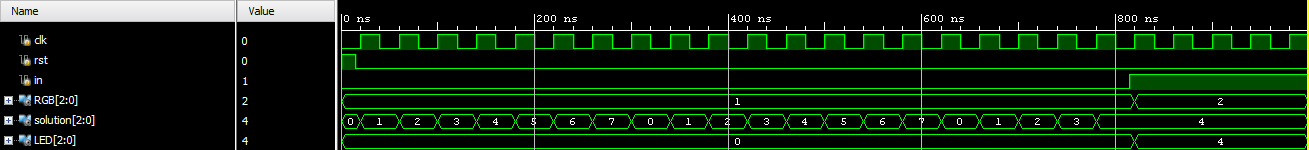
\includegraphics[width=\textwidth]{Images/waveform_solver}
    \caption{Waveform output of \c{Solver.v}.}
    \label{waveform:solver}
\end{figure}

Figure \ref{waveform:solver} shows the waveform for \c{Solver.v}.
Its function is to loop through the numbers 0 to 7 and back
again until it detects a 1 from its input \c{in}. When it does,
it stops looping and sets the output \c{LED} to the value
it found a 1 for. Additionally, the output \c{RGB} goes from
1 (representing red) to 2 (representing green).

\begin{figure}[H]
    \centering
    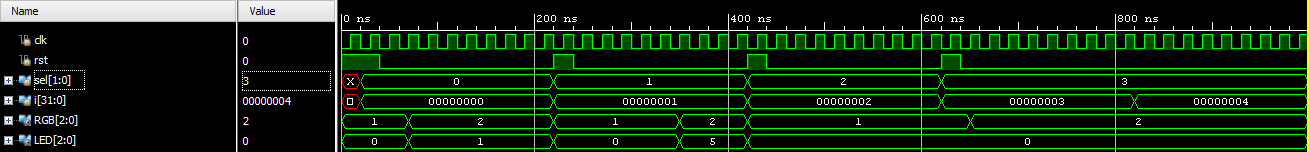
\includegraphics[width=\textwidth]{Images/waveform}
    \caption{Waveform output of \c{top\_level\_mod.v}v}
    \label{waveform:toplevelmod}
\end{figure}

Figure \ref{waveform:toplevelmod} shows the waveform for
\c{top\_level\_mod.v}. Just as before, an easy indicator
to see whether a function has been satisfied is the
\c{RGB} output: 1 means ``no'', and 2 means ``yes''.
All functions are indeed satisfiable except Function 2
(where \c{sel} is 2).

Below are pictures of all four functions. Note that
Function 2 is unsatisfiable and therefore its light is red.

\begin{figure}[H]
    \centering
    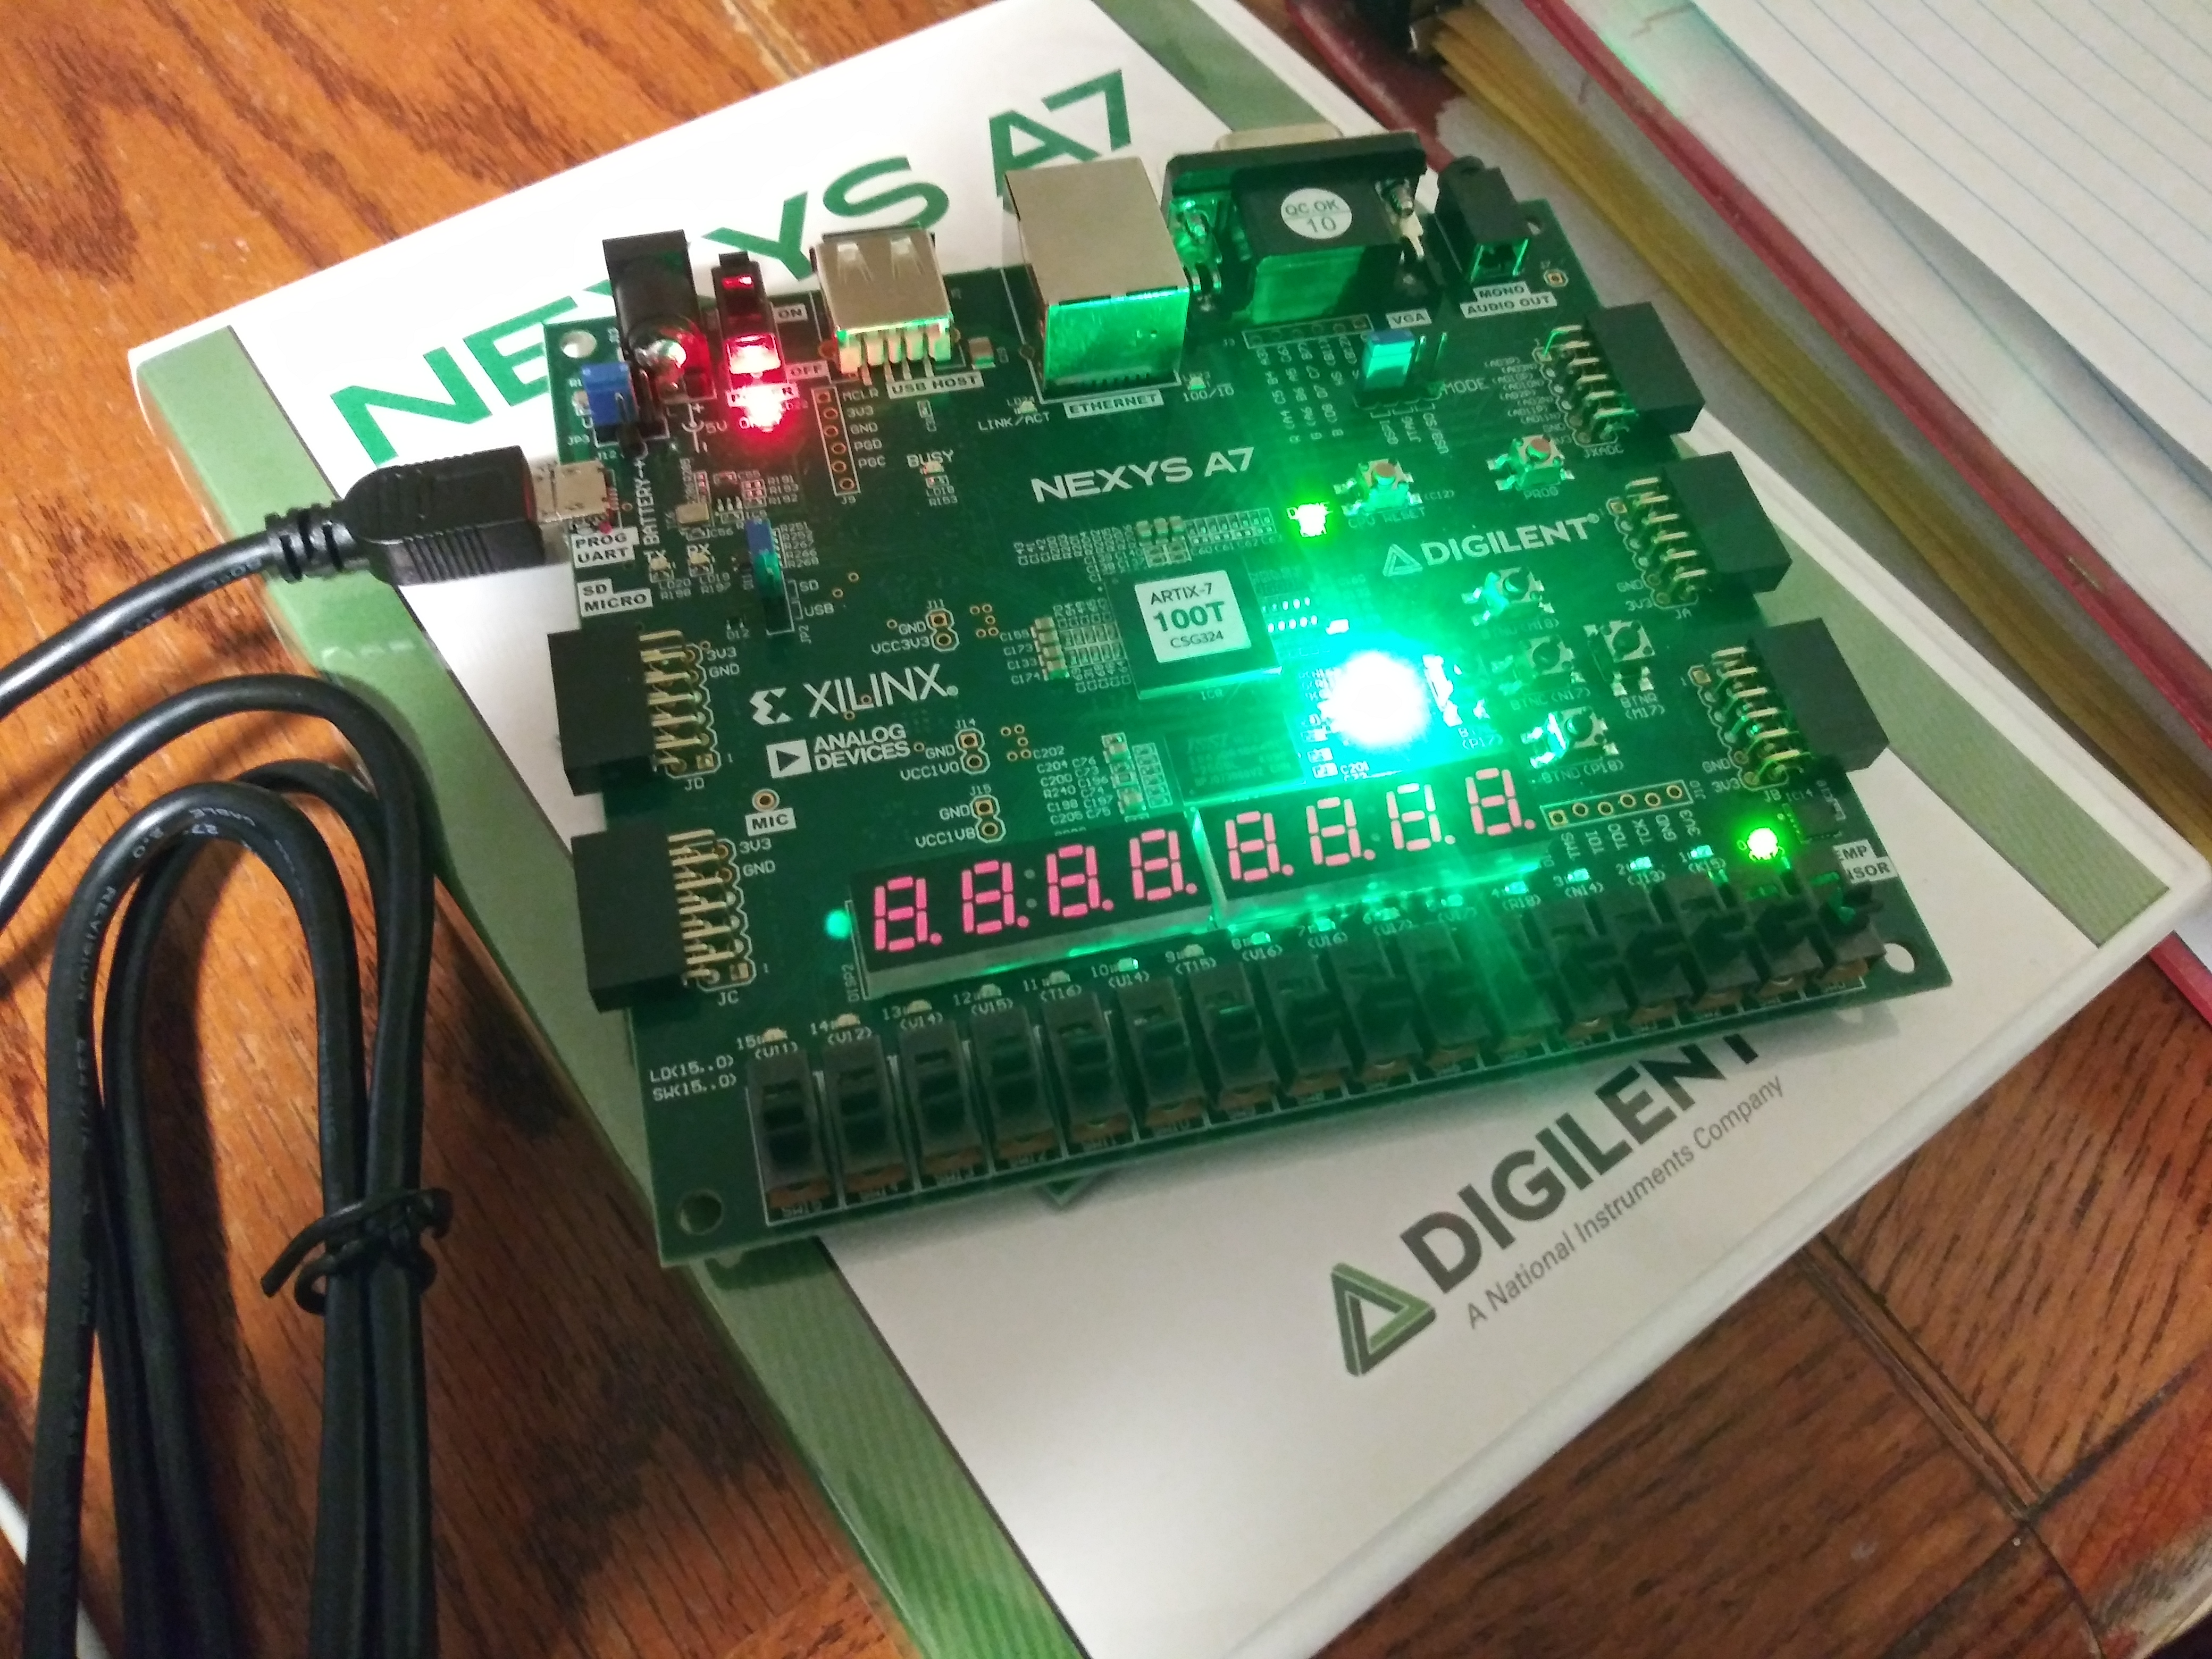
\includegraphics[width=\textwidth]{Images/0}
    \caption{Function 0.}
    \label{pic:func0}
\end{figure}

\begin{figure}[H]
    \centering
    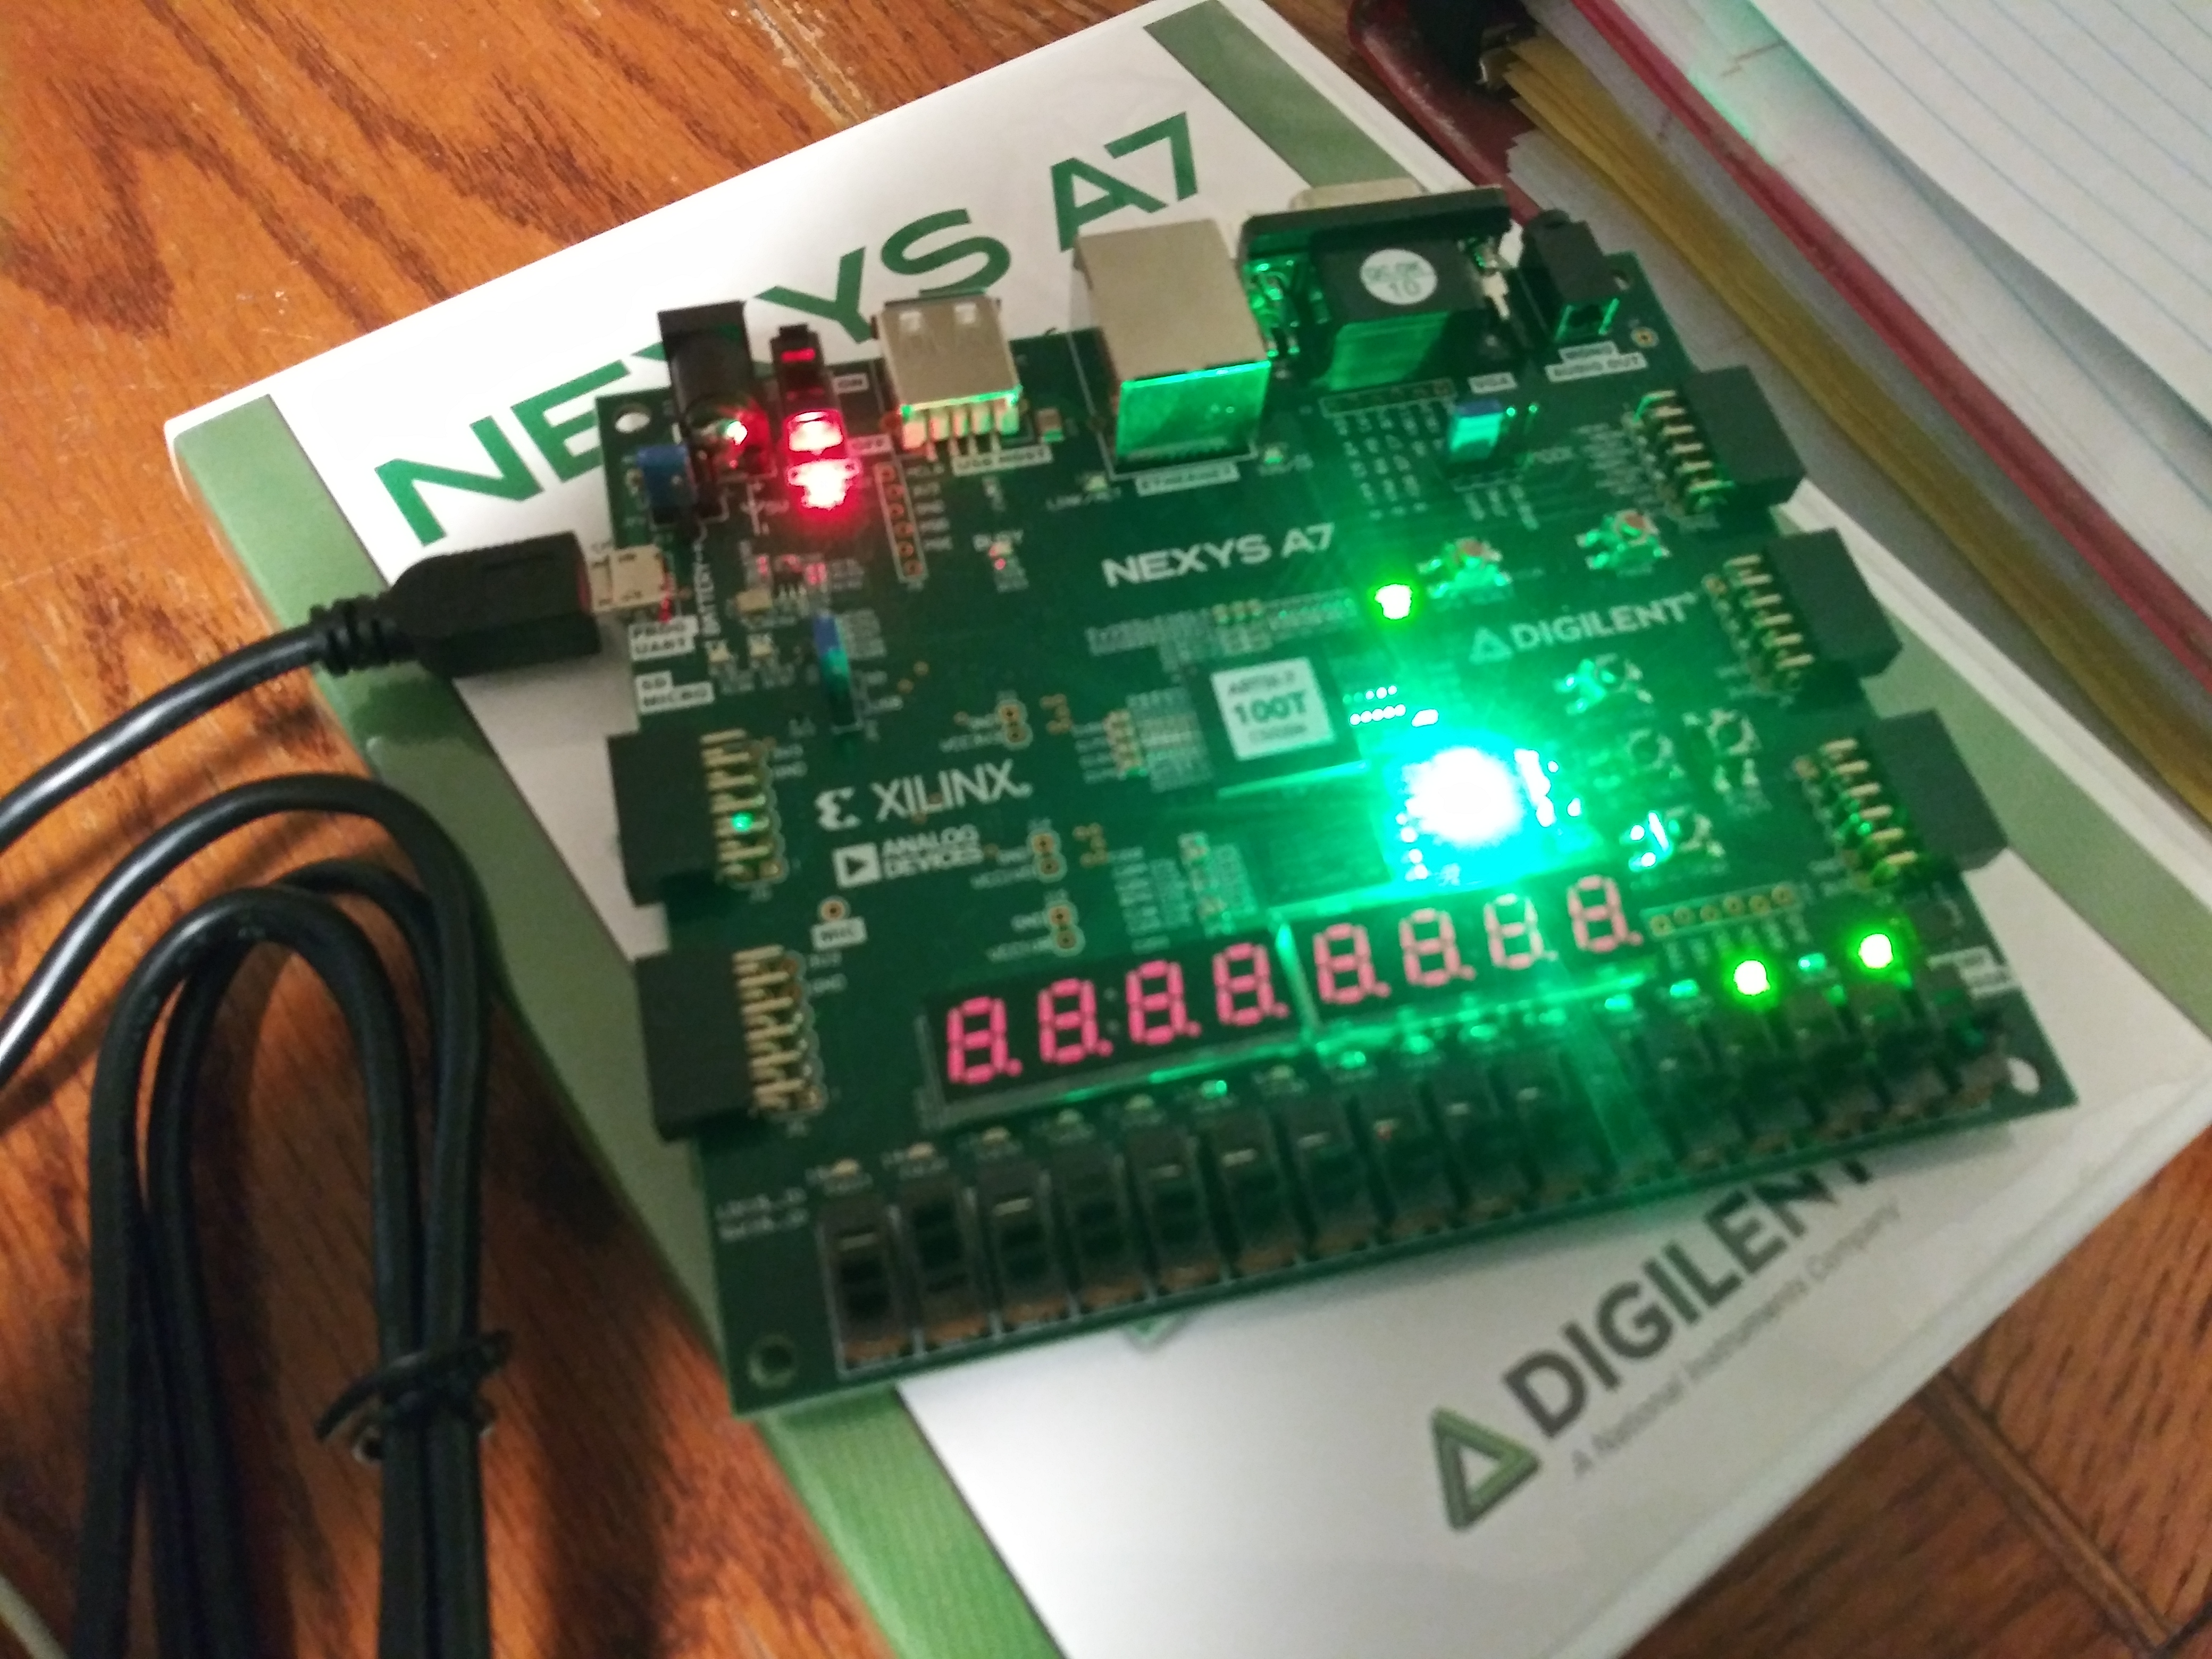
\includegraphics[width=\textwidth]{Images/1}
    \caption{Function 1.}
    \label{pic:func1}
\end{figure}

\begin{figure}[H]
    \centering
    \includegraphics[width=\textwidth]{Images/2}
    \caption{Function 2.}
    \label{pic:func2}
\end{figure}

\begin{figure}[H]
    \centering
    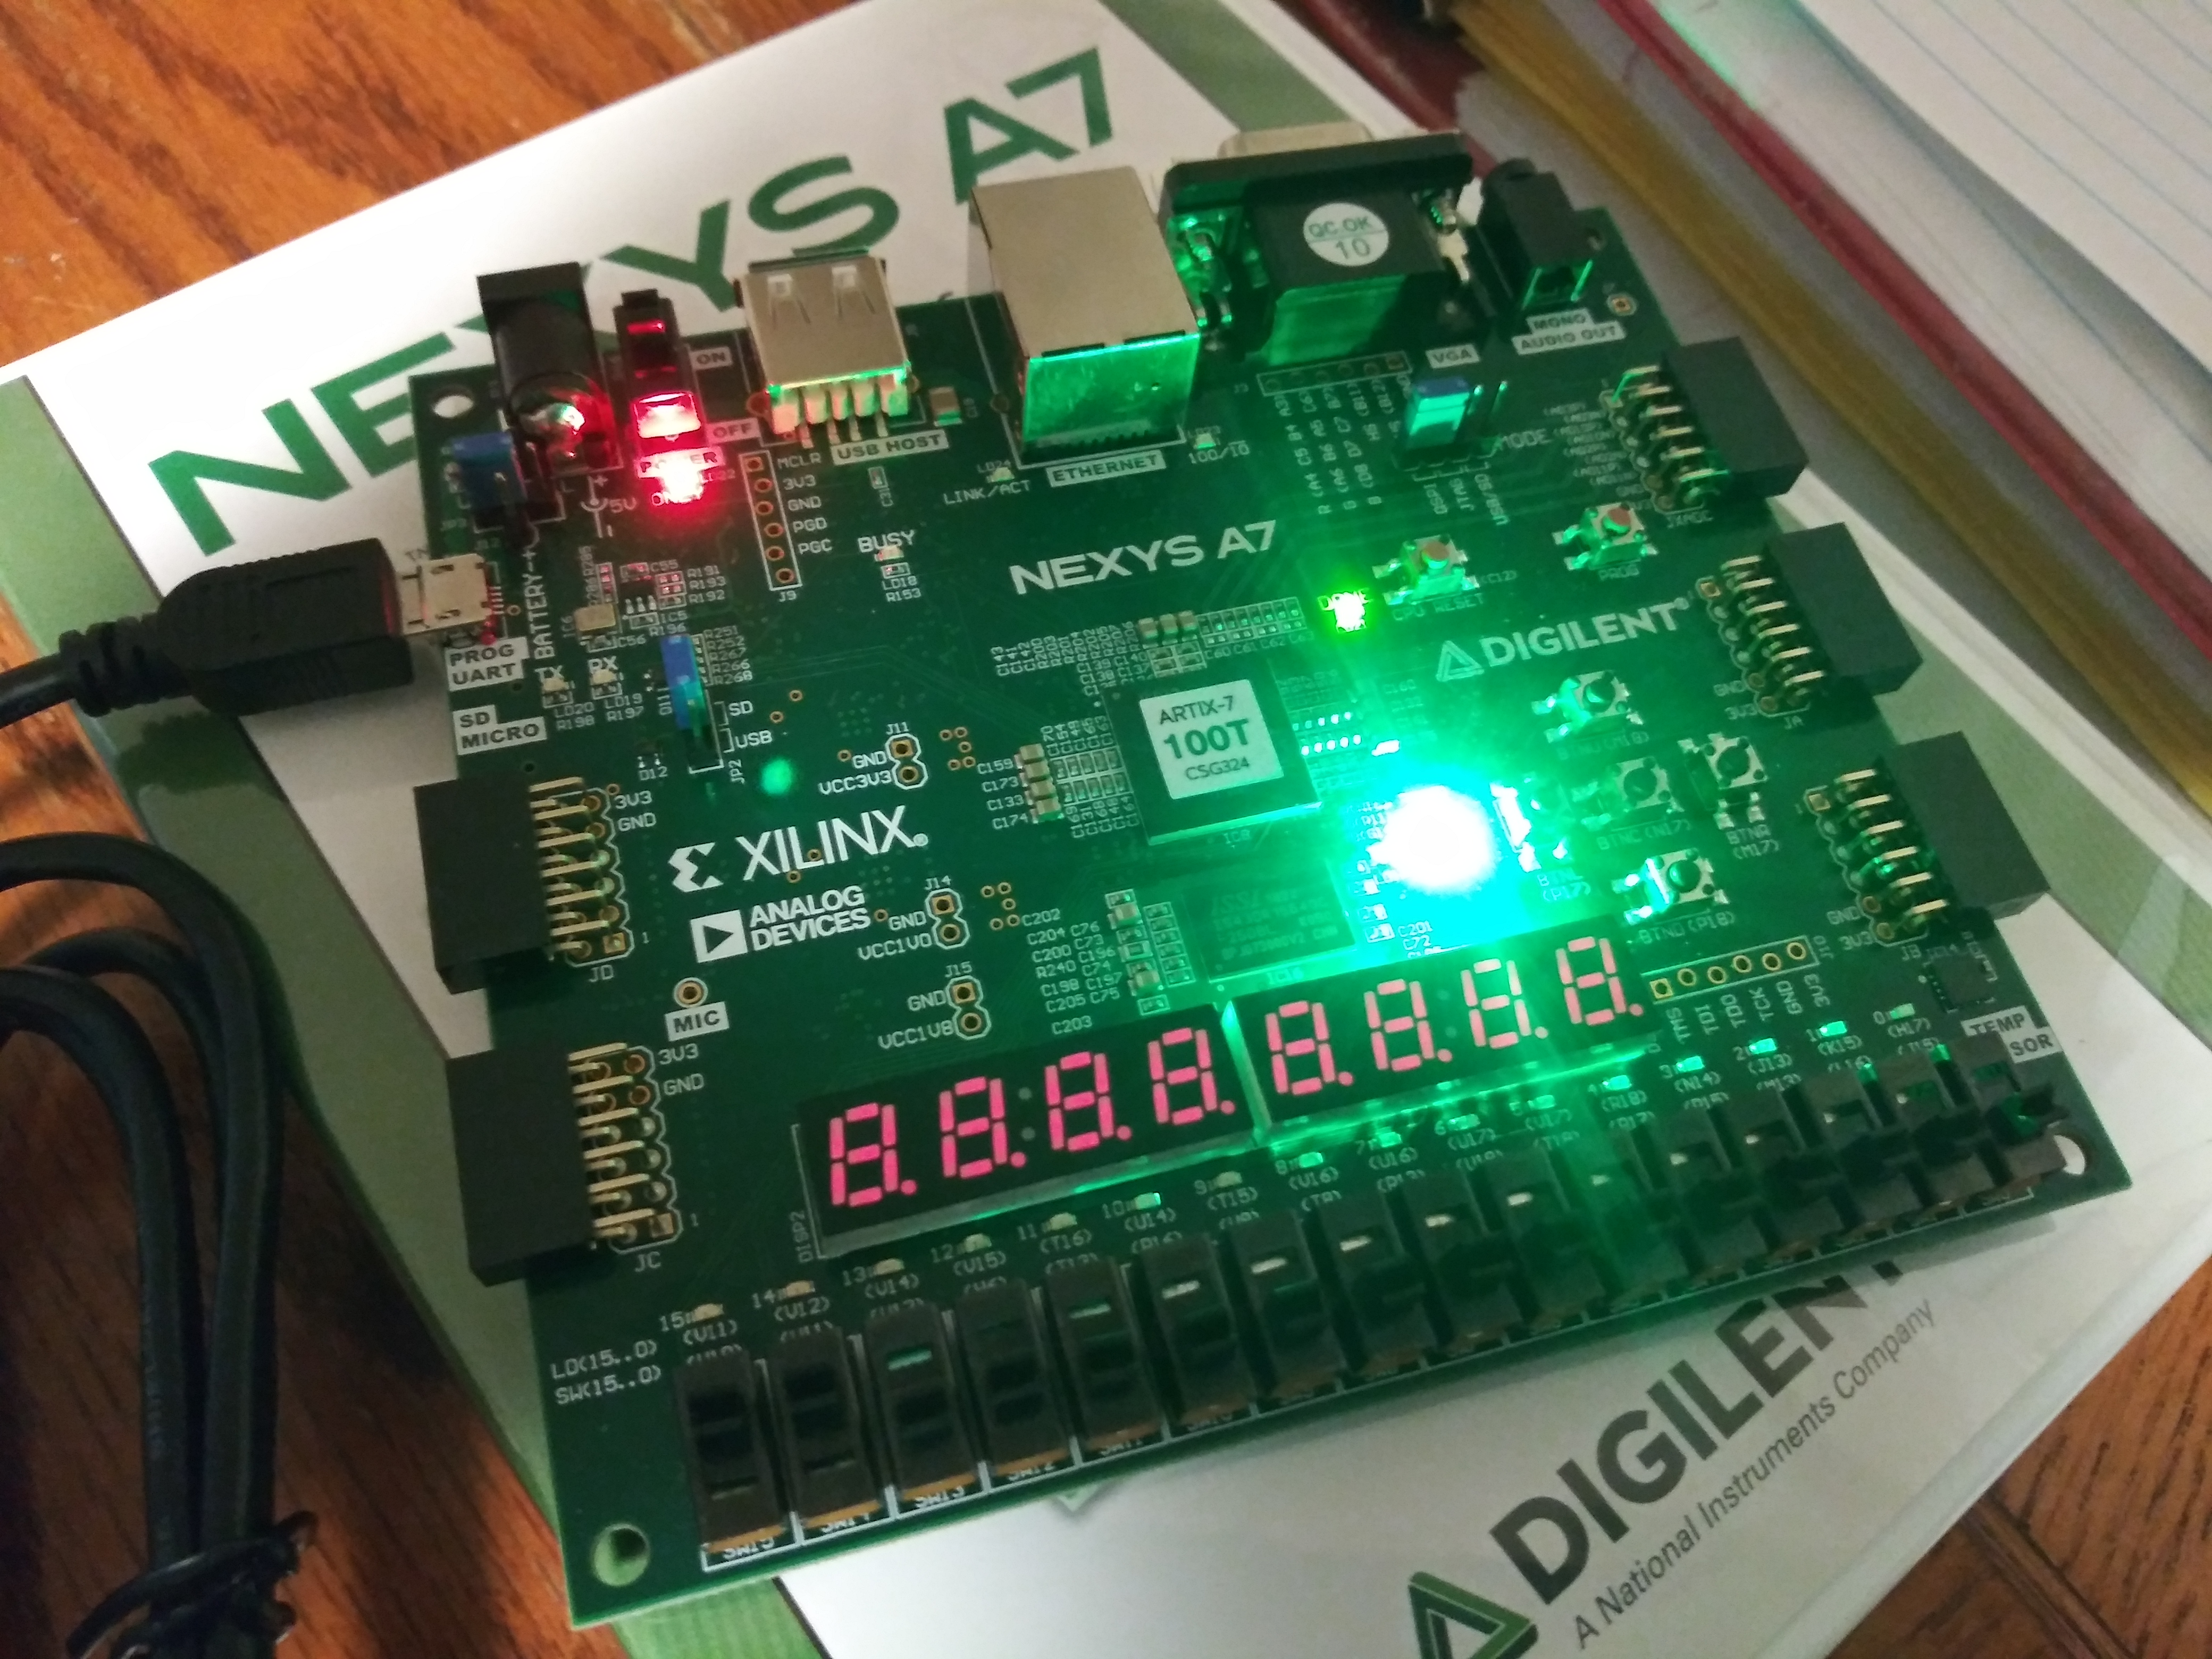
\includegraphics[width=\textwidth]{Images/3}
    \caption{Function 3.}
    \label{pic:func3}
\end{figure}

\end{document}
